\documentclass[
  a4paper,
  12pt,
  oneside,
  parskip=half,
  listof=totoc,
  bibliography=totoc,
  DIV=12,
  numbers=noenddot
  ]{scrartcl}

% ========== Grundlegende Kodierung & Schriften ==========
\usepackage[utf8]{inputenc}
\usepackage[T1]{fontenc}           % Für LuaLaTeX: ermöglicht Systemfonts und Unicode

% ========== Seitenlayout ==========
\usepackage[
  a4paper,
  left=2.0cm,       % Linker Rand = 2.5cm
  right=2.0cm,    % Rechter Rand = 2.5cm
  top=2.0cm,      % Oberer Rand = 2.5cm
  bottom=2.5cm,   % Unterer Rand = 3cm
  footskip=1.25cm,   % Abstand Fußzeile
  %bindingoffset=5mm % Bindungskorrektur
]{geometry}

\usepackage[onehalfspacing]{setspace}   % 1.5-facher Zeilenabstand
%\renewcommand*\familydefault{\sfdefault} % Serifenlose Schriftart
\usepackage{lmodern}               % Latin Modern Schrift (skalierbare Vektorfonts)
\usepackage[babel]{microtype}             % Verbesserte Textformatierung

% ========== Kopf- und Fußzeilen für scrreprt ==========
%\usepackage[headsepline]{scrlayer-scrpage}
%\automark[section]{chapter}   % inner header = section, outer = chapter
%\\textbf{}setkomafont{pagehead}{\normalfont}
%\pagestyle{scrheadings}
%\clearpairofpagestyles
%\ihead{\leftmark}    % inner header = Kapitel
%\ohead{\pagemark}    % outer header = Seitenzahl


% ========== Bibliographie ==========
\usepackage[
  backend=biber,       % Biber als Backend
  style=numeric-comp,       % Physik-Stil (AIP/APS Standard)
  sorting=none,        % Sortiere nach Reihenfolge des Auftretens im Text
  maxnames=3,         % Maximale Namen vor "et al."
  minnames=2          % Minimale Namen vor "et al."
  %doi=false,
  %url=false,
  %isbn=false
  ]{biblatex}
\DeclareFieldFormat{titlecase}{#1} % Titel in Groß- und Kleinschreibung
\AtEveryBibitem{\clearfield{note}} %Weglassen von note
\AtEveryBibitem{\clearfield{pagetotal}} %Weglassen von Seitenzahlen
\DeclareFieldFormat[article]{journaltitle}{\textit{#1}} %Journal kursiv
\DeclareNameAlias{author}{family-given} %Reihenfolge Nachmane, Vorname tauschen
\DefineBibliographyStrings{english}{andothers = {\textit{et al\adddot}}} %et al. kursiv
\DeclareFieldAlias{journaltitle}{shortjournal} % Use shortjournal if available for abbreviated journal titles

\addbibresource{ResearchProject.bib} %Bibliographie-Datei einbinden


% ========== Sprach- & Zeitoptionen ==========
\usepackage[english]{babel}
\usepackage{csquotes}            % Für korrekte Anführungszeichen (automatisch an Sprache angepasst)

% ========== Naturwissenschaftliche Pakete ==========
\usepackage{amsmath}
\usepackage{amssymb}
\usepackage{mathtools}
\usepackage{bm}
\usepackage{fixmath}
%\usepackage{unicode-math}
\usepackage{physics}
%\usepackage{mhchem}            % Chemische Formeln
\usepackage[locale=DE]{siunitx} % SI-Einheiten mit deutschen Standards
\sisetup{
  output-decimal-marker = {,}, % Komma als Dezimaltrennzeichen
  per-mode = fraction,         % Einheiten als Bruch
  group-separator = {.},       % Tausendertrenner (Punkt)
  range-units = single         % Einheiten bei Bereichen: \SI{5-10}{\meter}
}
\DeclareSIUnit\pixel{px}


% ========== Grafikpakete ==========
\usepackage{graphicx}
\usepackage{pdfpages}               % PDF Impoort
%\usepackage{svg}
\usepackage{float}                  % Präzise Positionierung von Abbildungen
\usepackage{wrapfig}                % Floating Text
\usepackage{tikz}                   % Erstellung von Diagrammen und Grafiken
\usepackage[font=footnotesize,labelfont=bf]{caption}
%\graphicspath{{./graphics}}

% ========== Tabellen ==========
\usepackage{array}                 % Erweiterte Tabellenfunktionen
\usepackage{booktabs}              % Professionelle Tabellenlinien
\usepackage{longtable}             % Mehrseitige Tabellen
\usepackage{multirow}              % Zellen über mehrere Zeilen
\setlength{\arrayrulewidth}{0.4mm} % Dicke der Tabellenlinien

% ========== Referenzen und Zitationen ==========
\usepackage{xurl}
\usepackage[colorlinks=true, urlcolor=black, linkcolor=black, anchorcolor=black, citecolor=blue]{hyperref}             
\usepackage[labelfont={bf}, labelsep=colon]{caption} % Anpassung von Bildunterschriften
\DeclareCaptionLabelSeparator{colon}{\space|\space} % Figurename | bei Abbildungen
\usepackage{subcaption}             % Unterbilder (a), (b), etc.
\usepackage{cleveref}

% ========== Benutzerdefinierte Befehle ==========
% Kurzbefehle für häufig verwendete Notationen
\newcommand{\di}{\partial}           % Partielle Ableitung (kurz)
\newcommand{\e}{\mathrm{e}}          % Euler's e (aufrecht)
\newcommand{\im}{\mathrm{i}}         % Imaginäre Einheit (aufrecht)
\newcommand{\dif}{\mathop{}\!\mathrm{d}} % Differential (richtige Abstände)
\newcommand{\HRule}{\rule{\linewidth}{0.5mm}} % Horizontale Linie (für Titelseite)
\newcommand{\ShouldBe}{\stackrel{\mathclap{\normalfont\mbox{!}}}{=}}


\begin{document}
	
\section{Problem}

\begin{figure}[H]
	\centering
	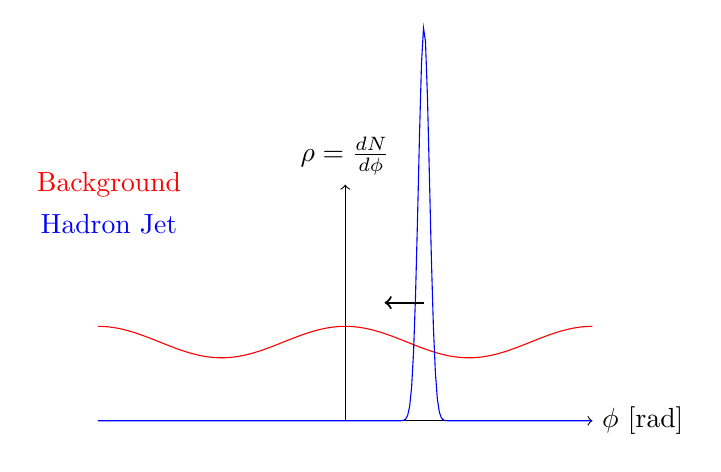
\begin{tikzpicture}
		%draw coordinate system
		\draw [->] (-3.14,0) -- (3.14,0)node[right] {$\phi$ [rad]};
		\draw [->] (0,0) -- (0,3) node[above] {$\rho = \frac{d N}{d \phi}$};
		%draw functions
		\draw [red] plot[domain=-3.14:3.14,
		samples = 50,
		smooth]({\x}, {1 + 0.2*cos((360/6.28)*2*\x)});
		\draw [blue] plot[domain=-3.14:3.14,
		samples = 250]({\x}, {5*exp(-((\x-1)*(\x-1))/0.01)});
		%draw labels
		\draw (-3,3) node[color=red] {Background};
		\draw (-3,2.5) node[color=blue] {Hadron Jet};
		%draw arrows
		\draw[->, thick](1,1.5)--(0.5,1.5);
		
	\end{tikzpicture}
	\caption{The particle densities of the background (subject to flow) and of the hadron jet.The jet is being produced independently form the underlying background. Because of how the anti-$k_t$ cluster-algorithm works, the jet is more probably clustered farther left than it is farther right.}
\end{figure}

We want to quantitatively investigate how far the jet is pulled based on how the flow underneath looks like. Since the jet radius is much smaller than the $v_2$ flow modulation, we can expand the underlying flow locally according to

\begin{equation}
	\begin{gathered}
		\rho_\text{BG}(\phi) |_{\phi_J} := \frac{d N}{d (\phi - \psi_m)} |_{\phi_J} \propto 1 + 2 \sum_{n \geq 1}^{} v_n \cos(n (\phi - \psi_m)) |_{\phi_0}\\
		\approx 1 + 2v_2 \cos(2(\phi - \psi_m)) |_{\phi_J} \\
		= \rho_0(\phi_J) + m \cdot (\phi - \phi_J) + \mathcal{O}(m^2) \text{ where } m \in \mathbb{R}
	\end{gathered}
	\label{eq:background_density}
\end{equation}

It is difficult to fully translate the anti-$k_t$ algorithm's behavior into an analytical model for many particles. That is why we will look at how the algorithm clusters a jet in the low-particle limit where only one high-$p_T$ jet particle is clustered with one low-$p_T$ particle in the thermal background. Its position is determined by where it appears most probably around the jet particle according to equation (\ref{eq:background_density}). This is sufficient to prove the first-order behavior in $m$. If the jet shift would depend on $m$ only in higher polynomial orders, the first particle would have to shift the jet by 0 also if $m \neq 0$.

\section{Coordinate System}

For simplicity, let us have the high-$p_T$ jet particle to have $\phi_J := 0$ and the particle to have $\phi_P$.

\begin{figure}[H]
	\centering
	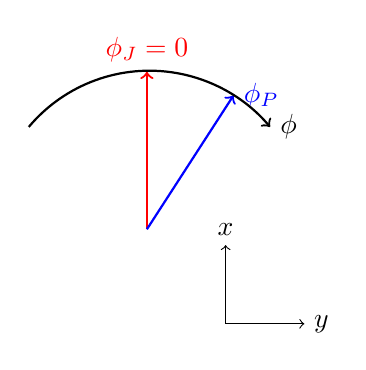
\begin{tikzpicture}
		
		% Particles
		\draw[thick , ->, red] (0,1) -- (0,3) node[above] {$\phi_J = 0$};
		\draw[thick , ->, blue] (0,1) -- (1.1,2.7) node[right] {$\phi_P$};
		
		% Winkelbogen oben
		\draw[thick, ->] (-1.5,2.3) arc[start angle=140,end angle=40,radius=2] node[right] {$\phi$};
		
		% Kleines Koordinatensystem unten rechts
		\begin{scope}[shift={(1,-0.2)}]
			\draw[->] (0,0) -- (0,1) node[above] {$x$};
			\draw[->] (0,0) -- (1,0) node[right] {$y$};
		\end{scope}
		
	\end{tikzpicture}
	\caption{The ALICE coordinate system with the jet particle (pseudo jet) at $\phi = 0$.}
\end{figure}

Therefore the four-momenta of the the particles are

\begin{equation}
	\begin{gathered}
		p_J^\mu = (E_J, p_{T,J}, 0, 0), \\
		p_P^\mu = (E_P, p_{T,P} \cos(\phi_P), p_{T,P} \sin(\phi_P), 0) \approx (E_P, p_{T,P} (1-\frac{\phi_P^2}{2}), p_{T,P} \phi_P, 0)
	\end{gathered}
\end{equation}

The new jet coordinate $\phi_*$ will be equivalent to the jet shift. 

\section{Clustering}

The anti-$k_t$ algorithm will cluster these two particles, adding up their four-momenta such that the four-momentum of the clustered jet is

\begin{equation}
	\begin{gathered}
		p_*^\mu = p_J^\mu + p_P^\mu = (E_J + E_P, p_{T,J} + p_{T,P}(1 - \frac{\phi_P^2}{2}), p_{T,P} \phi_P, 0) .
	\end{gathered}
\end{equation}

The azimuthal coordinate of the clustered jet $\phi_*$ can be calculated by using the geometric relation between $\phi, p_x, p_y$

\begin{equation}
	\begin{gathered}
		\phi_* \approx \tan(\phi_*) = \frac{p_*^2}{p_*^1} = \frac{p_{T,P} \phi_P}{p_{T,J} + p_{T,P} (1-\frac{\phi_P^2}{2})} \approx \frac{p_{T,P} \phi_P}{p_{T,J} + p_{T,P} } \propto \phi_P
	\end{gathered}
\end{equation}

\section{The BG particle's position $\phi_P$}

The BG particle is generated based on $\rho_{BG}(\phi)$ in proximity to the jet within a jet radius $R$. Other values are also possible, it does not affect the proportionality property. The average coordinate of the BG particle can be calculated based on

\begin{equation}
	\begin{gathered}
		<\phi_P> = \frac{\int_{-R}^{R} d\phi \, \phi \, \rho_{BG}(\phi)}{\int_{-R}^{R} d\phi \,  \rho_{BG}(\phi)} \propto \int_{-R}^{R} d\phi \, \phi \, (\rho_0 + m \phi + \mathcal{O}(m^2)) = \frac{2}{3} m R^3 + \mathcal{O}(m^2)) \propto m
	\end{gathered}
\end{equation}

\section{Conclusion}

Thus, we can conclude that

\begin{equation}
	\begin{gathered}
		\phi_* \propto \phi_P \propto m = \frac{d \rho_{BG}(\phi)}{d \phi} |_{\phi_J} = - 4 v_2 \sin(2(\phi - \psi_m)) |_{\phi_J}
	\end{gathered}
\end{equation}

where $m$ is the first derivative of the particle flow density and we are left with fit parameters $(A, \psi_m)$:

\begin{equation}
	\begin{gathered}
		\phi_* = A \sin(2(\phi - \psi_m))
	\end{gathered}
\end{equation}

\end{document}